We now study stability and finite-particle error for the general mean-field system
\eqref{eq:general_mf_system_opt}--\eqref{eq:general_mf_system_x}. In order to do this, given two solutions $(\vartheta_t,\nu_t),(\tilde{\vartheta}_t,\tilde{\nu}_t)$, we define the distance metric \citep{pgd_theory}
\begin{equation*}
    \mathbf{d}((\vartheta_t,\nu_t),(\tilde{\vartheta}_t,\tilde{\nu}_t)):=\sqrt{\|\vartheta_t-\tilde\vartheta_t\|^2
    +
    W_2^2(\nu_t,\tilde\nu_t)},
\end{equation*}
and introduce the main assumptions required for our convergence results.

\begin{assumption}[Twisted joint strong monotonicity]\label{ass:twisted_joint_strong_monotonicity}
Suppose that there exist symmetric positive definite matrices $D_\vartheta$ and $D_z$, and a constant $\rho>0$, such that, for every $t\ge0$, every $\vartheta,\tilde\vartheta\in\Theta\times\sM$, every $\nu,\tilde\nu\in\mathcal P_2(\sX\times\sV)$, and every coupling $\Lambda\in\Gamma(\nu,\tilde\nu)$, the following inequality holds:
\begin{align}
&\left\langle \vartheta-\tilde\vartheta,\,
    D_\vartheta
    \left[
    \Psi_t(\vartheta,G_\nu(\vartheta))
    -
    \Psi_t(\tilde\vartheta,G_{\tilde\nu}(\tilde\vartheta))
    \right]
    \right\rangle \notag\\
&\quad+
\int
\Big[
    \left\langle z-\tilde z,\,
    D_z
    \left[
    b_{\Pi_\theta(\vartheta)}(z)
    -
    b_{\Pi_\theta(\tilde\vartheta)}(\tilde z)
    \right]
    \right\rangle \notag\\
&\quad+
    \frac{1}{2}\left\|
    D_z^{1/2}
    \left[
    \sigma_{\Pi_\theta(\vartheta)}(z)
    -
    \sigma_{\Pi_\theta(\tilde\vartheta)}(\tilde z)
    \right]
    \right\|_{\mathrm{HS}}^2
\Big]\Lambda(\mathrm dz,\mathrm d\tilde z) \notag\\
&\le
-\rho\left(
    \|\vartheta-\tilde\vartheta\|_{D_\vartheta}^2
    +
    \int\|z-\tilde z\|_{D_z}^2\,
    \Lambda(\mathrm dz,\mathrm d\tilde z)
\right).
\label{eq:joint_strong_monotonicity_twisted}
\end{align}
\end{assumption}
\ref{ass:twisted_joint_strong_monotonicity} is the contractivity condition for the coupled optimiser--sampler system in the twisted metrics \(\|\cdot\|^2_{D_\vartheta}\) and \(\|\cdot\|^2_{D_z}\). When \(D_\vartheta=I_{d_\theta+d_m}\) and \(D_z=I_{d_x+d_v}\), it reduces to the usual joint dissipativity condition in the product Euclidean metric.

\begin{remark}
\ref{ass:twisted_joint_strong_monotonicity} is a genuinely joint
contractivity condition: dissipativity of the exact-gradient optimiser and
of each frozen sampler does not by itself suffice;
Appendix~\ref{app:cross_assumptions} provides an explicit counterexample.  Appendix~\ref{app:separated_assumptions} gives a componentwise
small-gain criterion that combines separate dissipativity and Lipschitz bounds
for the optimiser response, gradient observation, sampler drift, and diffusion
through a positive-definite cross-coupling matrix.
Appendix~\ref{app:cor_projected_strong_convexity} instead gives a structured
criterion based on strong monotonicity of a projected field
\(\Phi=(F,\nabla_xE)\), or joint strong convexity of an underlying potential
when this field is conservative, together with sufficient dissipation of the
auxiliary variables. Finally, Appendix~\ref{app:mpgd_result} gives a concrete
hypocoercive construction for a heavy-ball optimiser coupled to an
underdamped sampler.
\end{remark}

\begin{theorem}\label{thm:twisted_joint_strong_monotonicity}
Suppose \ref{ass:strong_sol_exist_unique} and \ref{ass:twisted_joint_strong_monotonicity} hold with positive definite matrices \(D_\vartheta,D_z\) and constant \(\rho>0\). Let \((\vartheta_t,\nu_t)\) and \((\tilde\vartheta_t,\tilde\nu_t)\) be any two solutions of \eqref{eq:general_mf_system_opt}--\eqref{eq:general_mf_system_x} with initial sampler laws in \(\mathcal P_2(\sX\times\sV)\). Define
\[
\kappa
:=
\frac{\lambda_{\max}(\mathrm{diag}(D_\vartheta,D_z))}
{\lambda_{\min}(\mathrm{diag}(D_\vartheta,D_z))}.
\]
Then, for every \(t\ge0\),
\begin{equation*}
\mathbf d((\vartheta_t,\nu_t),(\tilde\vartheta_t,\tilde\nu_t))
\le
\sqrt{\kappa}\,e^{-\rho t}
\mathbf d((\vartheta_0,\nu_0),(\tilde\vartheta_0,\tilde\nu_0)). 
\end{equation*}
If, in addition, \ref{ass:existence_minimizer} holds, define
\(\mu_t:=\delta_{\vartheta_t}\otimes\nu_t\) and
\(\mu_\star:=\delta_{\vartheta_\star}\otimes\nu_{\theta_\star}\).
Then, for every initial product law
\(\mu_0=\delta_{\vartheta_0}\otimes\nu_0\), with
\(\nu_0\in\mathcal P_2(\sX\times\sV)\),
\[
W_2(\mu_t,\mu_\star)
\le
\sqrt{\kappa}\,e^{-\rho t}W_2(\mu_0,\mu_\star).
\]
Consequently, \(\mu_\star\) is the unique finite-second-moment stationary law among laws of the form \(\delta_\vartheta\otimes\nu\). For time-dependent \(\Psi_t\), stationary means that initializing from the law leaves the law unchanged for every \(t\ge0\).
\end{theorem}
The proof can be found in Appendix~\ref{app:thm_joint_strong_monotonicity}. We now consider bounding the error between the particle approximation and the mean-field system. For this, we follow \citet{pgd_theory} and introduce an auxiliary $N$-copy mean field system. Let \(\bar\vartheta_0\) be deterministic, and let
\(\bar Z_0^1,\ldots,\bar Z_0^N\) be i.i.d.\ with common law
\(\bar\nu_0\in\mathcal P_2(\sX\times\sV)\), independently of the mutually independent Brownian motions $(B_t^1,\ldots,B_t^N)_{t\ge0}$. Defining the system
\begin{align}
    \mathrm d\bar\vartheta_t
    &=
    \Psi_t(\bar\vartheta_t,G_{\bar\nu_t}(\bar\vartheta_t))\,\mathrm dt,\qquad\qquad\qquad \label{eq:n-copy-1}\\
    \mathrm d\bar Z_t^i
    &=
    b_{\Pi_\theta(\bar\vartheta_t)}(\bar Z_t^i)\,\mathrm dt
    +
    \sigma_{\Pi_\theta(\bar\vartheta_t)}(\bar Z_t^i)\,\mathrm dB_t^i,
    \label{eq:n-copy-2}
\end{align}
then \(\bar\vartheta_t\) is deterministic and
\(\bar Z_t^1,\ldots,\bar Z_t^N\) are i.i.d.\ with common law \(\bar\nu_t\). We define the empirical measure $\bar\nu_t^{[N]}$ of the $N$-copy system as $\bar\nu_t^{[N]}=({1}/{N})\sum_{i=1}^N\delta_{\bar Z_t^i}$. We now state further assumptions that are required for our parameter error bound.
\begin{assumption}[Lipschitz gradient response]\label{ass:psi_F_lipschitz}
Assume that $\Psi_t$ is uniformly Lipschitz in its gradient argument: for all
$t\ge0$, all $\vartheta\in\Theta\times\sM$,
$g,\tilde g\in\mathbb R^{d_\theta}$,
\[
    \|\Psi_t(\vartheta,g)-\Psi_t(\vartheta,\tilde g)\|
    \le
    L_\Psi\|g-\tilde g\|.
\]
\end{assumption}

\begin{assumption}[Uniform gradient fluctuation]\label{ass:mf_bounded_second_moment}
Assume the mean-field copy system defined in \eqref{eq:n-copy-1}--\eqref{eq:n-copy-2} has uniformly bounded variance of the stochastic gradient:
\[
    \sup_{t\ge0}
    \mathbb E
    \left[
    \left\|
    F(\Pi_\theta(\bar\vartheta_t),\Pi_x(\bar Z_t))
    -
    G_{\bar\nu_t}(\bar\vartheta_t)
    \right\|^2
    \right]
    \le
    V_F
    <
    \infty.
\]
\end{assumption}
{\color{red}\ref{ass:mf_bounded_second_moment}}
is a uniform variance bound for the stochastic-gradient integrand.  It follows,
for example, if \(F(\theta,\cdot)\) is globally Lipschitz with a Lipschitz
constant uniform in \(\theta\) and
\(\sup_{t\geq0}\mathbb E\|\Pi_x(\bar Z_t)\|^2<\infty\).  More generally, a
linear-growth bound uniform along the optimiser path, together with the corresponding uniform second-moment bounds, is sufficient.

\begin{theorem}[Finite-particle interaction error]
\label{thm:finite_particle_error}
Suppose \ref{ass:strong_sol_exist_unique}, \ref{ass:twisted_joint_strong_monotonicity}--\ref{ass:mf_bounded_second_moment} hold.
Let $(\vartheta_t^N,Z_t^1,\ldots,Z_t^N)$ solve the particle system
\eqref{eq:general_particle_system_opt}--\eqref{eq:general_particle_system_x}
with the same Brownian motions and the synchronous initial conditions
\(\vartheta_0^N=\bar\vartheta_0\) and \(Z_0^i=\bar Z_0^i\).
Let \((\bar\vartheta_t,\bar Z_t^1,\ldots,\bar Z_t^N)\) solve the \(N\)-copy mean-field system \eqref{eq:n-copy-1}--\eqref{eq:n-copy-2}. Then, for every
$t\ge0$,
\[
    \Ltwonorm[\big]{\mathbf{d}\big((\vartheta^N_t,\nu_t^N),(\bar\vartheta_t,\bar\nu_t^{[N]})\big)}
    \le
    \tfrac{L_\Psi}{\rho}
    \sqrt{\tfrac{\kappa V_F}{N}}
    \left(1-e^{-\rho t}\right),
\]
where $\kappa$ is the condition number of
$\mathrm{diag}(D_\vartheta,D_z)$.
\end{theorem}
The proof is given in Appendix~\ref{app:proof_finite_particle_error} and proceeds as a generalisation of Lemma 13 in \cite{pgd_theory}. Using Theorems \ref{thm:twisted_joint_strong_monotonicity} and \ref{thm:finite_particle_error}, we may provide a full parameter error bound of the particle system \eqref{eq:general_particle_system_opt}--\eqref{eq:general_particle_system_x}.

\begin{theorem}[Parameter error bound of particle system]\label{thm:parameter_error_full}
    Suppose \ref{ass:strong_sol_exist_unique}--\ref{ass:mf_bounded_second_moment} hold. Assume \(\vartheta_0^N\) is deterministic and \(Z_0^1,\ldots,Z_0^N\) are i.i.d.\ with common law \(\nu_0\), independently of the mutually independent Brownian motions. Then the $\mathrm{L}^2$ parameter error satisfies
\begin{equation*}
\Ltwonorm{\theta^N_t-\theta_\star}\le \sqrt{\kappa}\,e^{-\rho t}
\mathbf d_0+\tfrac{L_\Psi}{\rho}
\sqrt{\tfrac{\kappa V_F}{N}}
\left(1-e^{-\rho t}\right),
\end{equation*}
with
\(\mathbf d_0:=\mathbf d((\vartheta^N_0,\nu_0),(\vartheta_\star,\nu_{\theta_\star}))\), the initial distance from the stationary mean-field solution. Consequently,
\begin{align*}
\lim_{N\to\infty}\limsup_{t\to\infty}
\Ltwonorm{\theta_t^N-\theta_\star}=0.
\end{align*}
\end{theorem}
The proof is given in Appendix~\ref{app:cor_parameter_error_full} and follows from Theorems~\ref{thm:twisted_joint_strong_monotonicity}--\ref{thm:finite_particle_error}. Theorem~\ref{thm:parameter_error_full} concerns the continuous-time particle
system. To describe at a high level how time discretisation would enter the
bound, let \(h>0\), let \(t_k:=kh\), and denote by
\(\widehat\theta_k^{N,h}\) the parameter iterate produced by a numerical
discretisation of the particle dynamics. Supposing the discretisation can
be coupled to the continuous-time system so that, for some error function
\(\varepsilon_{\mathrm{disc}}\) such that $\Ltwonorm{\widehat\theta_k^{N,h}-\theta_{t_k}^N}
\leq
\varepsilon_{\mathrm{disc}}(h,t_k,N),
$
where \(\varepsilon_{\mathrm{disc}}(h,t_k,N)\to0\) as \(h\to0\) -- for example,
on each finite horizon \(T\), one may have
\(\sup_{t_k\leq T}\varepsilon_{\mathrm{disc}}(h,t_k,N)
\leq C_T h^\alpha\) for some \(\alpha>0\).  The triangle inequality then gives the end-to-end estimate
\begin{align*}
\Ltwonorm{\widehat\theta_k^{N,h}-\theta_\star}
\leq
\Ltwonorm{\theta_{t_k}^N-\theta_\star}
+
\varepsilon_{\mathrm{disc}}(h,t_k,N),
\end{align*}
where the first term is bounded by Theorem~\ref{thm:parameter_error_full}.
Establishing such sampler- and optimiser-specific discretisation rates,
especially uniformly over an infinite time horizon, requires a separate
stability and numerical-analysis argument.  We leave this to future
work, since the primary aim of the paper is to demonstrate the
framework and establish its theoretical foundations.
\glsunset{mypgd}
\glsunset{myholpgd}
\begin{figure*}[t!]
\centering
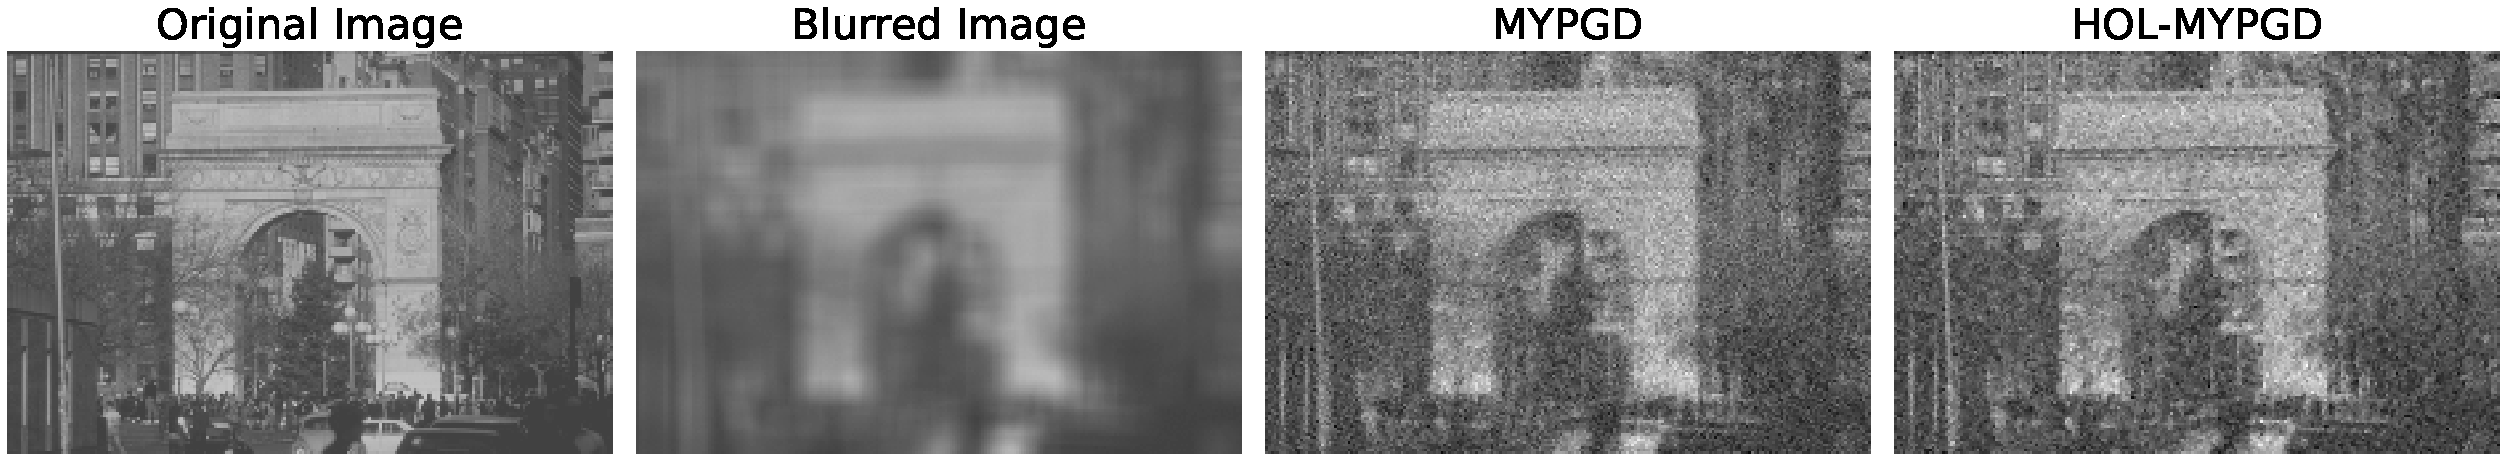
\includegraphics[width=1.0\textwidth]{images/mmle/mmle_deblurring_image_maintext.pdf}
\caption{Ground truth (left), blurred image (middle-left), and comparisons to single particle reconstructions produced by methods \gls*{mypgd} (middle-right) and \gls*{myholpgd} (right) for setup A.}
\label{fig:deblurring_example}
\end{figure*}